\chapter{Introduction}
\label{chap:intro}

Having to plan dinner while on a tight schedule or a tight budget can be a menace, especially if you crave something in particular. In other situations, you just want a low-cost dinner to save money, especially if you are a student, or near the end of the month where money is tight. But what recipes can you make?\\
It is not really hard to find an exciting recipe with ingredients that suit your taste as there are tons of different web services and applications for that. These are usually simple and fast to use, however they are not always completely unbiased. Companies tend to launch big recipe applications for their specific line of products. An example could be the application \emph{`Karolines Køkken'}\cite{arla}, which recommends recipes with Arla products as ingredients.\\ A lot of different big danish companies like \textit{Arla}, \textit{Amo} or \textit{Dan Sukker} have custom fitted applications for their field of interests. \\
There are some great free applications, based on user uploaded recipes with a possibility to rate them such as \emph{`Opskrifter.dk'}\cite{opskrifterdk}. These applications provide easy lookup of recipes in different categories, but without price and ingredient searching. \\
Applications for searching on groceries or ingredients exist, but they do not incorporate recipes. There are a couple of applications such as \emph{`eTilbudsavisen}\cite{etilbudsavis}. These applications gathers offers from different catalogs, providing users with the cheapest ingredients in nearby stores. If a user wants to find the price of a certain recipe, he would have to search each ingredient individually. If the ingredients are not on sale, he has to know the price in a certain store beforehand. It is completely unreasonable to believe a person can remember every price for each product for each of the retailers.


\section{Existing Software}
\label{sec:exsoft}

As mentioned there are a couple of existing software solutions that solves parts of the problem base we have earlier established. There are a lot of different recipe applications or websites and to mention a few; Food Network in the Kitchen \cite{recipe_FN}, Woman's Day 100 Budget Meals \cite{recipe_woman}, Slow Copper Recipes \cite{recipe_SC} and Supercook \cite{recipe_supercook}. What all of these have in common is that they provide recipes based on certain premises, whether it is based on certain equipment such as a slow cooker or it is based on cheap meals. \\
Neither of these have a location based system -in the best case, they only provide recipes and a estimate of the costs based on online stores. All of the above mentioned are however American examples, and of course there are plenty of danish applications built on the same concept. In America it is possible to find prices of staple goods online as it is possible to order things from regular grocery retailers, but that is not possible in Denmark. It is sometimes possible to search by brand in many of the applications but none of them have automatic comparison of nearby grocery stores. In Denmark we have an existing service, the before mentioned eTilbudsavis \cite{etilbudsavis}. This service gathers information from catalogs the stores send out themselves, and tags all advertised products. It allows the user to create a wish list/shopping list and figure out if the items are on sale from different retailers. It furthermore uses maps to keep store locations, which means you have the possibility to see nearby stores and what they offer. This application does however not have recipe support, meaning you can not compare recipes and give estimates on the prices. As it is only based on offers, it is even difficult to give estimates on most full recipes, even if you wanted to.

\section{The idea}
\label{sec:theidea}

The idea appeared as part of the daily life of a normal student. Students in general, do not have a large budget for buying luxury ingredients to make interesting meals. However, eating pasta and ketchup seven days a week is not fun. So the motivation for this project was how to plan something interesting for dinner while staying on a low budget. 

The problem can be solved by using two existing software solutions, but we found no application that combines the two, to make a complete service.

Below is listed two motivational scenarios for making this application, and show . The first is: you just got off the university and you walk into a grocery store to pick up items to make dinner. You are tired and have trouble working out what to make. This is when you pull out your mobile phone and open Billig Aftensmad. The application knows your taste and uses GPS-location to figure out which grocery store you are in. It will now provide you with a list of recipes matching your taste and searching criteria, from which you can gain inspiration or fully commit to cooking a certain recipe. The application will give you a list of ingredients to buy, and how to prepare and cook the meal.

The second scenario is: you are sitting a home planing your dinners for the following week. You are trying to make ends meet on a low budget, therefore you want to buy cheap meals but additionally want some healthy and quality food. You use Billig Aftensmad to search for cheap recipes in a five kilometer radius around your place and you look where you can pick the ingredients for these recipes up, saving the most possible money. It is optional, but if you want the application to help you picking healthy food, you search for the recipe tag \textit{healthy}, and you will be provided with healthy recipes.

\begin{figure}[H]
	\centering
	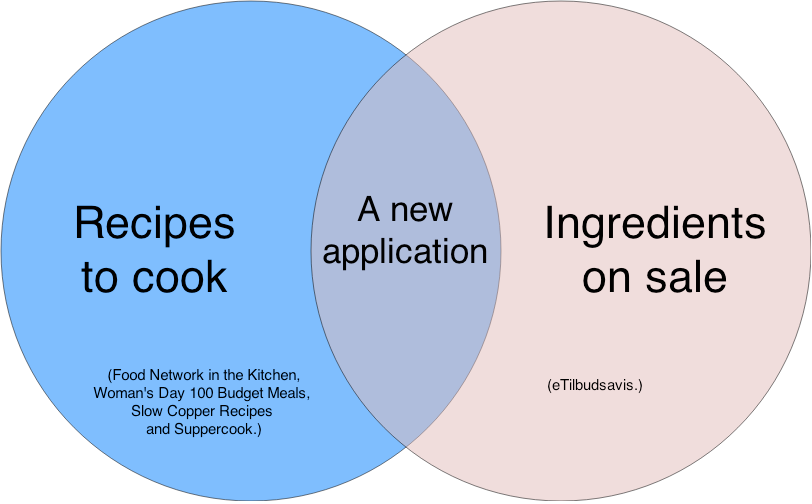
\includegraphics[width=0.7\textwidth]{Pictures/theideadiagram.png}
	\caption{Diagram showing the coupling of two fields, to make a new innovative application.}
	\label{fig:theideaasdiagram}
\end{figure}

The motivation for this application is providing existing services in a combined form and attach more opportunities regarding search, sorting and preferences to this combined application. Figure \ref{fig:theideaasdiagram} shows how the two existing services are coupled to form a new application.
\section{Problemstatement}
\label{sec:probstate}

Something along these lines

\emph{How can we produce a recipe application which focuses on cheap offers from nearby retail stores}


